\chapter %\chapter[<ToC-title>]{<Title>}
[Morphing Polylines Based on Least-Squares Adjustment]
{Morphing Polylines\\ Based on Least-Squares Adjustment}
\label{chap:Morph}


Digital maps such as Google Maps or OpenStreetMap have become 
one of the most important sources of geographic information. 
When users interactively browse through such maps on computers 
or small displays, they often need to zoom in and out to get the 
information desired. Often, zooming is supported by a multiple 
representation database (MRDB). 
This database stores a discrete set of levels of detail (LODs), 
from which a user can query the LOD for a 
particular scale \parencite{Hampe2004multiple}. 
A small set of LODs, however, leads to 
large and sudden changes during zooming, 
which distracts users.
Therefore, hierarchical schemes have been proposed that 
implement the generalization process 
based on small incremental changes, 
for example, the binary line generalization tree 
(BLG-tree) \parencite{vanOosterom2005} 
for line simplification 
or the generalized area partitioning tree (GAP-tree)
\parencite{vanOosterom1995GAPTree} 
for area aggregation. 
The incremental generalization process is 
represented in a data structure 
that allows a user to retrieve a map at any desired scale. 
Still, the generalization process 
consists of discrete steps and includes abrupt changes. 
To achieve a continuous generalization, 
\textcite{Sester2004} simplified building footprints 
based on small incremental steps 
and smoothly animated each step. 
Also aiming at a continuous generalization, 
several authors have developed 
methods for morphing between two polylines
\parencite{Cecconi2003,Noellenburg2008}. 
Most of these methods consist of two steps 
\parencite{Cecconi2003,Noellenburg2008,Peng2012River}. 
The first step is to compute the corresponding points
of the two polylines. 
The second step is to define a trajectory for each 
pair of corresponding points. 
Most often, straight lines are used as trajectories.
Then, morphing is realized by moving points 
along the straight-line trajectories with constant speeds.

In this chapter, we relax the requirement of using
straight-line trajectories for morphing.
Our concern with straight-line trajectories is that 
characteristics (e.g., bends) of the polylines 
can change drastically during a morphing process. 
To better keep the characteristics, 
we suggest that the angles and the edge lengths of polylines 
should change linearly during a morphing process. 
As \figs\ref{fig:Morph_LengthChanging}a and 
\ref{fig:Morph_LengthChanging}b show, this is clearly 
not accomplished with straight-line trajectories. In contrast, 
the new method that we present in this chapter yields a 
close-to-linear relationship, for example, between time and edge 
lengths; see \figs\ref{fig:Morph_LengthChanging}c and 
\ref{fig:Morph_LengthChanging}d.

\begin{figure}[tb]
	\captionsetup[subfigure]
	{justification=centering,font=normalsize}
	\begin{subfigure}[b]{.49\textwidth}
		\centering
		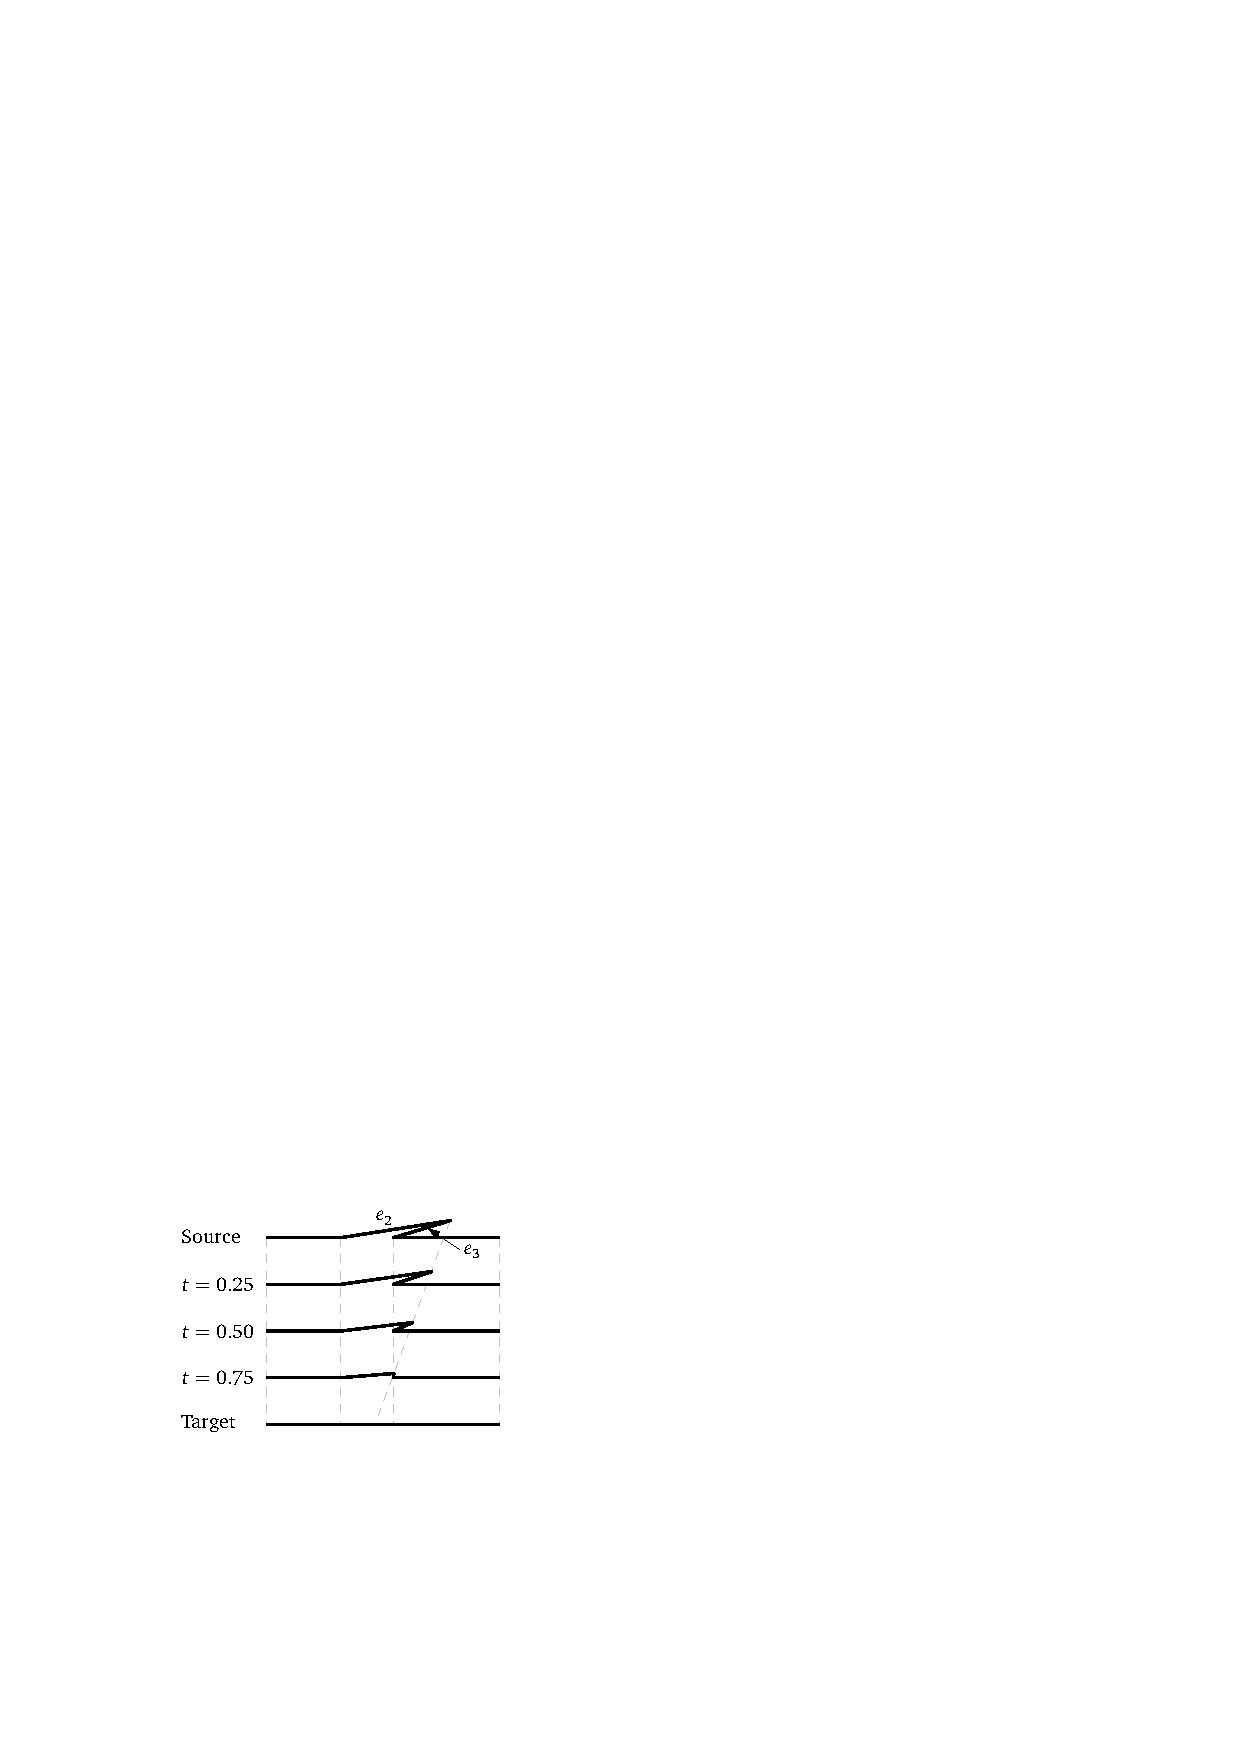
\includegraphics[page=1]{Morph_LengthChanging_Morph}
		\caption{\textbf{(a)}}
	\end{subfigure}
	\hfill
	\begin{subfigure}[b]{.49\textwidth}
		\centering
		
\includegraphics[page=1]{Morph_LengthChanging}
		\caption{\textbf{(b)}}
	\end{subfigure}

\bigskip
	\begin{subfigure}[b]{.49\textwidth}
	\centering
	\includegraphics[page=2]{Morph_LengthChanging_Morph}
	\caption{\textbf{(c)}}
\end{subfigure}
\hfill
\begin{subfigure}[b]{.49\textwidth}
	\centering
	
\includegraphics[page=2]{Morph_LengthChanging}
	\caption{\textbf{(d)}}
\end{subfigure}
	\caption{Morphing between 
		a source polyline and a target polyline.
		When morphing based on straight-line trajectories (a), 
		edge~$e_3$ receives almost zero length 
		at time~$t=0.75$ and then grows again (b). 
		With our method (c), 
		the edge lengths change almost linearly (d).}
	\label{fig:Morph_LengthChanging}
\end{figure}

The chapter is organized as follows. 
We review related work in 
\sect\ref{sec:Morph_RelatedWork}. 
The details of our method are presented in 
\sect\ref{sec:Morph_Methodology}, 
which include soft constraints, hard constraints, 
estimates for the unknowns, 
and the iterative process of our method. 
We present a case study in 
\sect\ref{sec:Morph_CaseStudy}, 
which shows that our 
method generally performs well but also reveals new problems. 
We conclude the chapter in 
\sect\ref{sec:Morph_Conclusion}.

\section{Related Work}
\label{sec:Morph_RelatedWork}

Different methods of morphing 
have been developed for map generalization. 
In map generalization, 
there are many constraints that need to be 
satisfied \parencite{Harrie1999}. 
These constraints should also be satisfied 
by intermediate-scale features displayed when morphing. 
According to \textcite{vanKreveld2001}, 
the amount of displacement 
between the corresponding vertices of two maps 
at different scales is quite small; 
thus, when using straight-line trajectories for morphing, 
hardly any features will be 
in conflict with the interpolated features. 
We, however, argue that even in simple situations, 
such as the one in 
\figs\ref{fig:Morph_LengthChanging}a and 
\ref{fig:Morph_LengthChanging}b, 
straight-line trajectories fail to 
generate satisfactory intermediate-scale features. 
In fact, there are methods that use curves rather than 
straight lines as vertex trajectories, 
for example, circular arcs or parabolas \parencite{Whited2009}. 
In contrast to these methods, our 
method does not require the trajectories to be of any particular 
curve type. 
Instead, we define the morphing process based on constraints 
that we impose on the features at intermediate scales.


Intermediate features are expected to be similar to 
the source feature and the target feature. 
We consider the angles and the edge lengths 
to be very important attributes of a feature, 
at least because similarity measures are often defined 
based on the angles and the edge lengths; 
\parencite[e.g.,][]{Arkin1991,Latecki2000,Frank2006}. 
\textcite{Sederberg1993} morphed two polygons by 
changing the angles and the edge lengths linearly over time. 
The authors also showed how to tweak 
the edge lengths and/or the angles to guarantee that
the intermediate polygon is closed at any time. 
We use an approach similar to \textcite{Sederberg1993}. 
We also try to achieve that 
the angles and the edge lengths change linearly. 
Unlike \textcite{Sederberg1993}, however, 
we simultaneously handle multiple constraints 
by defining (and solving) the model of a 
least-squares adjustment. 
A completely different approach was 
taken by \textcite{Connelly2003}. 
They proved that any polyline can be straightened, that is,
the vertices can be moved to a straight line 
such that the edge lengths never change and 
the edges never intersect. 
\textcite{Streinu2000} showed that 
a quadratic number of moves suffices 
and presented how to compute those. 
However, in order to morph a polyline into another polyline 
(with the same edge lengths), 
\textcite{Streinu2000} would morph the former
into a straight line and then into the latter. 
Thereby, that method will significantly change the angles.

Least-squares adjustment (LSA) has been shown to be effective 
in handling multiple constraints in map generalization
\parencite{Sester2000,Harrie2002}. 
Basically, it relies on 
function~$\phi: R^u \rightarrow R^m$ 
that defines the relationship between
vector~$\hat{X}$ of~$u$ \emph{unknowns} and 
vector~$L$ of~$m$ \emph{observations}. 
Given function~$\phi$ and vector~$L$, 
it is reasonable to ask for 
vector~$\hat{X}$ that strictly satisfies~$L=\phi(\hat{X})$. 
Such a vector, however, 
normally does not exist since~$m$ is usually larger than~$u$. 
Therefore, the \emph{corrections for observations}, 
vector~$v$, is introduced. 
Then, our aim is to find~$\hat{X}$ and~$v$ such that
\begin{equation}
L+v= \phi(\hat{X}), \nonumber
\end{equation}
and~$v^T P v$ is minimal, 
where~$P$ is a matrix 
that allows us to set weights to observations.
LSA is particularly easy to solve 
if a linear relationship between the unknowns 
and the observations exists, that is,
\begin{equation}
\label{eq:Morph_Relationship}
\phi(\hat{X})=A\hat{X}+d,
\end{equation}
where both matrix~$A$ and vector~$d$ have constant values. 
An optimum solution is given with
\begin{equation}
\label{eq:Morph_Solution}
\hat{X}=X_0+ (A^\mathrm{T}PA)^{-1}A^\mathrm{T}Pl,
\end{equation}
where \emph{estimates}~$X_0$ can be 
any vector of dimension~$u$ and vector~$l=L- \phi(X_0)$.

If the relationship 
between the unknowns and the observations is not linear,
then we have to compute iteratively 
in order to find an approximation of vector~$\hat{X}$. 
In this case, matrix~$A$ is defined based on 
the partial derivatives of function~$\phi$ at~$X_0$.
Usually, \eq\ref{eq:Morph_Solution} yields 
an approximation of the optimum 
unknown vector that is better than~$X_0$. 
A good approximation of~$\hat{X}$ can be 
found by iteratively solving \eq\ref{eq:Morph_Solution}. 
In each iteration (except the first),
we assign the newly computed vector,~$\hat{X}$, 
to vector~$X_0$.
Before we start the iteration, we should choose
a set of initial estimates that is close to~$\hat{X}$. 
The smaller the difference between~$X_0$ and~$\hat{X}$ is,
the more likely we find an approximation of~$\hat{X}$.

Since eighty percent of all objects (points, lines, and areas) 
in a typical medium-scale topographic map consist of lines
\parencite{Muller1991}, 
we focus on morphing polylines in this paper.


\section{Methodology}
\label{sec:Morph_Methodology}
In this section, we present our LSA-based morphing method. 
We introduce some 
definitions in \sect\ref{sec:Morph_Preliminaries}. 
Then, we model multiple requirements as constraints. 
The soft constraints are presented in 
\sect\ref{sec:Morph_SoftConstraints}. 
We set constant values to the coordinates of some 
vertices to implement hard constraints in 
\sect\ref{sec:Morph_HardConstraints}. 
The estimates for the unknowns are given in 
\sect\ref{sec:Morph_Estimates}. 
Finally, we sketch the stop condition of the model in 
\sect\ref{sec:Morph_Iterative}.

\subsection{Preliminaries}
\label{sec:Morph_Preliminaries}
Suppose that we have
polyline~$B$ with vertices~$b_1, \dots,b_M$ and 
polyline~$C$ with vertices~$c_1,\dots,c_N$, 
where~$B$ and $C$ represent the same geographic feature. 
Vertices~$b_1$ and~$c_1$ as well as~$b_M$ and~$c_N$ correspond 
to each other (see \fig\ref{fig:Morph_Injection}a). 
For every vertex of~$B$, we find a corresponding point (not 
necessarily a vertex) on~$C$, and vice versa. 
As a result, we have two new polylines, i.e., $B'$ and $C'$,
which have the same number, say $n$, of vertices
(see \fig\ref{fig:Morph_Injection}b).
How to find the corresponding pairs of vertices 
is not discussed in this chapter. 
We apply an algorithm similar to
\textcite{Noellenburg2008}, 
but any other method could be used as well.
\begin{figure}[tb]
	\centering	
	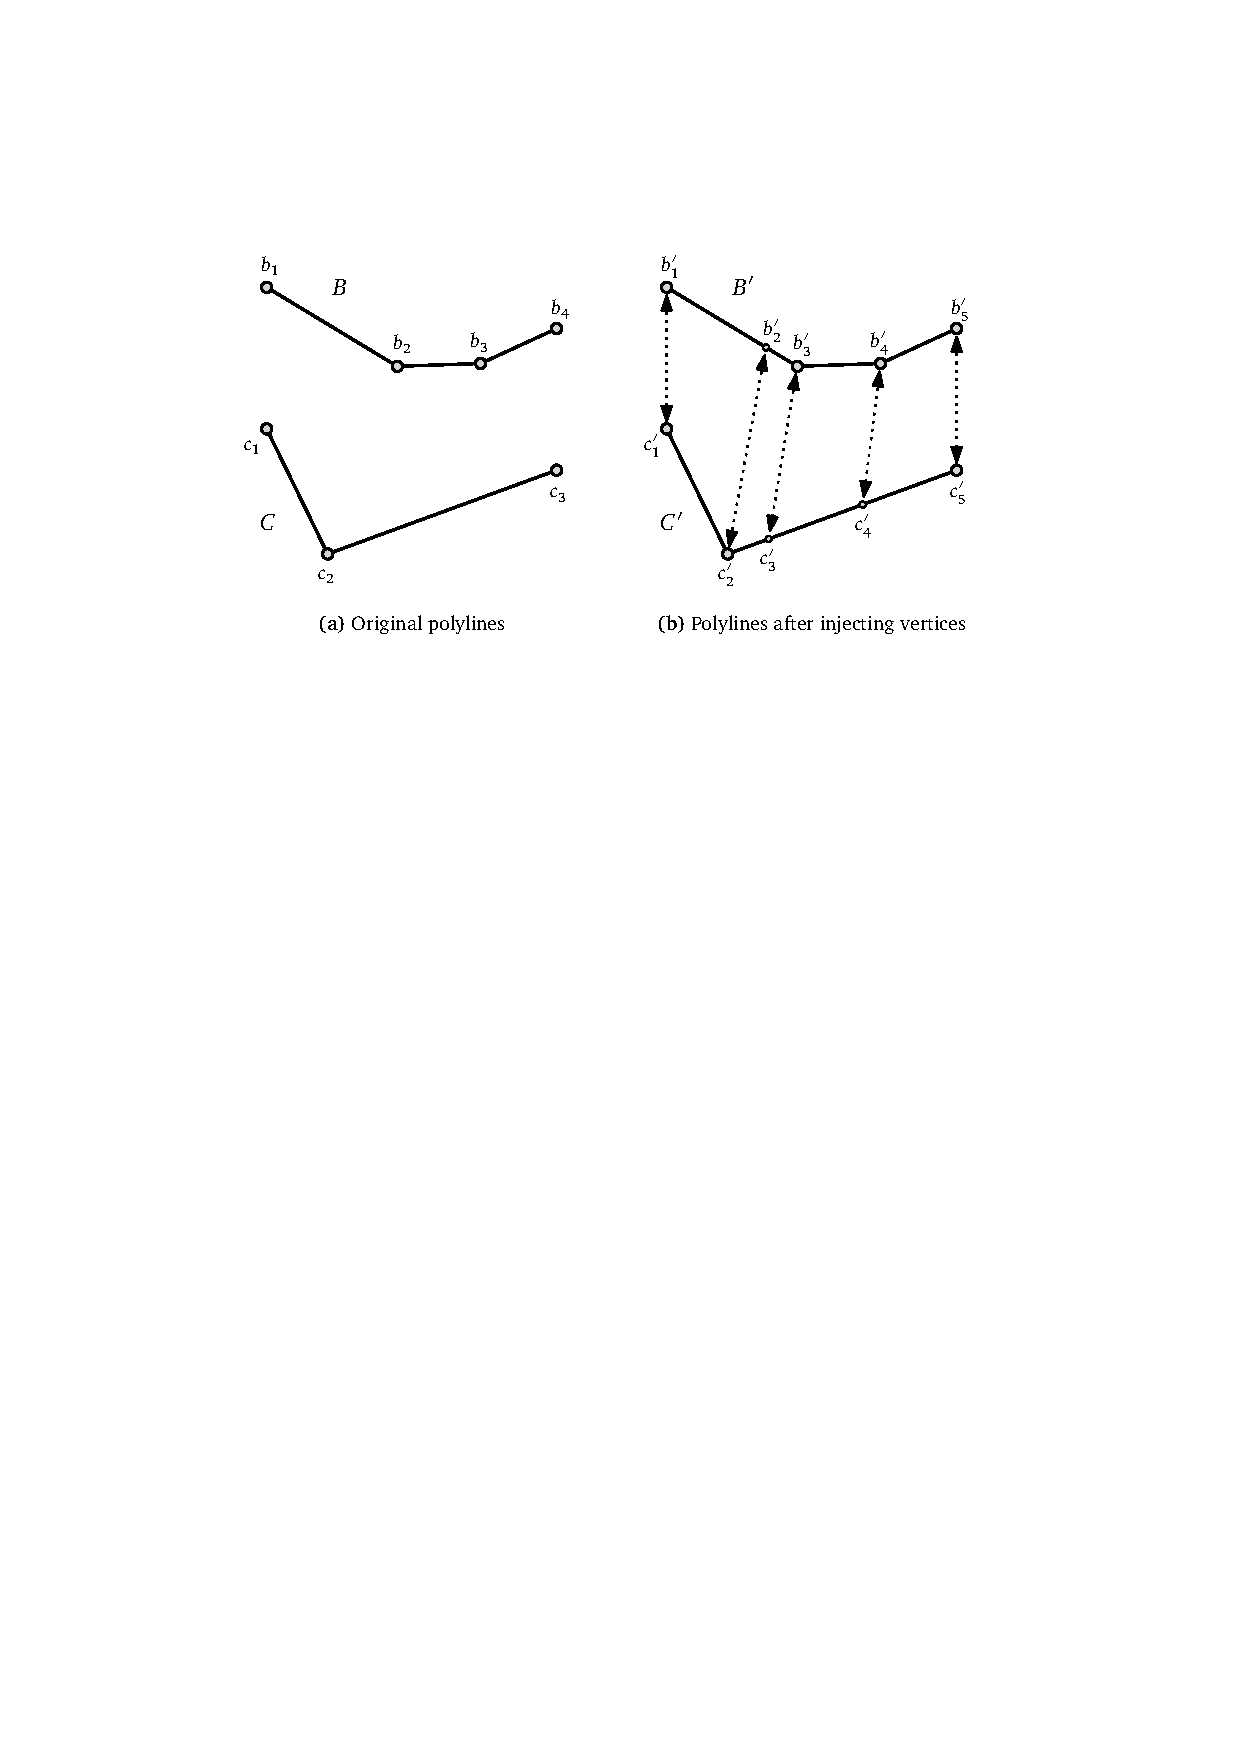
\includegraphics[page=1]{Morph_Methodology}
	\caption{Illustration of corresponding vertices.}
	\label{fig:Morph_Injection}
\end{figure}



The morphing process starts at time~$t=0$, from polyline~$B'$, 
and ends at time~$t=1$, to polyline~$C'$. 
Generally, we denote the polyline 
displayed at time~$t$ by~$D(t)$, 
thus~$D(0)=B'$ and~$D(1)=C'$. 
We denote the~$i$-th vertex of~$D(t)$ by~$d_i (t)$.


\subsection{Soft constraints}
\label{sec:Morph_SoftConstraints}
We compute polyline~$D(t)$ by constraining its 
angles and the lengths of its edges. 
That is, for each angle and each edge length, 
we define an expected value, 
which is an \emph{observation} in LSA. 
In most cases, 
these expected values cannot be achieved at the same time 
because they may contradict with each other. 
Therefore, we require that
the computed angles and edge lengths 
are close to the expected values. 
More precisely, we obtain the differences 
between the computed values and the expected values,
then we square the differences and sum up the squares;
we want to minimize the sum.
These requirements for angles and edge lengths 
constitute soft constraints in our method.
In order to make polylines behave as in our motivating example 
(see \figs\ref{fig:Morph_LengthChanging}c 
and~\ref{fig:Morph_LengthChanging}d), 
we define the expected values by a linear interpolation 
between the values of 
the source polyline and the target polyline. 
For the angles, the expected values are
\begin{equation}
\label{eq:Morph_AngleConstraints}
\beta_i(t)=(1-t)\cdot \beta_i(0) + t\cdot\beta_i(1),
\end{equation}
where $i=2,\ldots,n-1$.
Angles~$\beta_i (0)$ and~$\beta_i (1)$ 
are respectively from polylines~$B'$ and~$C'$ 
(see \fig\ref{fig:Morph_InitialsFinals}).

Similarly, for the edge lengths, we define
\begin{equation}
\label{eq:Morph_LengthConstraints}
l_i(t)=(1-t) \cdot l_i(0)+t\cdot l_i(1),
\end{equation}
where $i=1,\ldots,n-1$.
Lengths~$l_i(0)$ and~$l_i(1)$
are respectively from polylines~$B'$ and~$C'$ 
(see \fig\ref{fig:Morph_InitialsFinals}).

\begin{figure}[tb]
	\centering	
	\includegraphics[page=2]{Morph_Methodology}
	\caption{Illustration of initials and finals.}
	\label{fig:Morph_InitialsFinals}
\end{figure}

By applying LSA, our aim is to compute the adjusted coordinates
of the vertices for polyline~$D(t)$.
Therefore, we need to express 
the relationships between the adjusted coordinates,
$\hat{x}_{1}(t),\hat{y}_{1}(t), \ldots,
\hat{x}_{n}(t),\hat{y}_{n}(t)$,
and the observations 
(i.e., the expected angles and the expected edge lengths).
In other words, the adjusted coordinates 
are our \emph{unknowns} for LSA.
In the following, we express the relationships.

\emph{Angles:} Angle~$\beta_{i}(t)$ can be computed based on 
the difference between edge~$e_{i - 1}$'s $x$-axis angle 
and edge~$e_{i}$'s $x$-axis angle. 
The $x$-axis angle of an edge is the angle that 
we rotate $x$-axis until it is parallel to the edge
(see some examples in \fig\ref{fig:Morph_AxisAngle}). 
Depending on the quadrants 
in which \(e_{i - 1}\) and \(e_{i}\) lie 
relative to the vertex $d_{i}(t)$, 
a multiple of \(\pi\) has to be added.
As a result, for the adjusted angle~$\hat{\beta}_{i}(t)$ 
of observation~$\beta_{i}(t)$,
we require that
\begin{equation}
\label{eq:Morph_AdjustedAngle}
\hat{\beta}_{i}(t) = 
\arctan\frac
{\hat{y}_{i+1}(t) - \hat{y}_{i}(t)}
{\hat{x}_{i+1}(t) - \hat{x}_{i}(t)} 
- 
\arctan\frac
{\hat{y}_{i}(t) - \hat{y}_{i-1}(t)}
{\hat{x}_{i}(t) - \hat{x}_{i-1}(t)} 
+
K_{i} \cdot \pi,
\end{equation}
where $K_{i}\in \mathbb{Z}$ 
is a constant that only depends on~$i$.
For the LSA, we have to compute the partial derivatives of 
$\hat{\beta}_{i}(t)$ with respect to the unknowns. 
These partial derivatives do not depend on the constant term
$K_{i} \cdot \pi$. 
Therefore, we can neglect it.

\begin{figure}[tb]
	\centering	
	\includegraphics[page=3]{Morph_Methodology}
	\caption{The $x$-axis angles of some edges.
		The thin line segments represent $x$-axes,
		and the thick ones represent some edges.
}
	\label{fig:Morph_AxisAngle}
\end{figure}

\emph{Edge lengths:} Each edge length is a Euclidean distance. 
Hence, for adjusted edge length~$\hat{l}_{i}(t)$, 
we require that
\begin{equation}
\label{eq:Morph_AdjustedLength}
\hat{l}_{i}(t) = 
\sqrt{
	(\hat{x}_{i + 1}(t) - \hat{x}_{i}(t))^2
	+ 
	(\hat{y}_{i + 1}(t) - \hat{y}_{i}(t))^2}.
\end{equation}

Here, \eqs\ref{eq:Morph_AdjustedAngle} 
and~\ref{eq:Morph_AdjustedLength} constitute
function~$\phi(\hat{X})$;
see \eq\ref{eq:Morph_Relationship}. 
Since functions~$\hat{\beta}_{i}$ 
and~$\hat{l}_{i}$ are not linear, 
we have to linearize them by computing partial derivatives
\parencite{Sester2000,Harrie2002}.

Without adding hard constraints to our model, 
there is no need for an adjustment. 
We can perfectly satisfy every soft constraint 
simply by creating a new polyline with 
the expected angles and the expected edge lengths. 
However, the new polyline can be very different 
from our source polyline and target polyline;
in order to avoid this problem,
we add hard constraints of
prescribing some end vertices of the new polyline.

\subsection{Hard constraints}
\label{sec:Morph_HardConstraints}

There may be some common characteristic vertices on 
polylines $B'$ and $C'$. 
These vertices should be kept during morphing. 
If we have vertices $d_{i}(0) = d_{i}(1)$
for some $i\in \{1,\ldots,n\}$, 
we require as hard constraints that vertices
$d_{i}(0) = d_{i}(t) = d_{i}(1)$ for time $t \in [0,1]$.
That is to say, for these characteristic vertices, 
we do not introduce unknowns in the LSA. 
Note that our method does not require 
the existence of such common characteristic vertices, 
but it can handle them.

Even if vertex~$d_{i}(0)$, on polyline~$B'$, 
does not have the exact same position 
as its corresponding vertex~$d_{i}(1)$, on polyline $C'$, 
we may want to constrain computed vertex~$d_{i}(t)$ 
to lie at a prescribed position. 
In particular, by prescribing the end vertices of 
some polylines that meet each other at these end vertices,
we can guarantee that these polylines always meet each other.
This is useful if we need to deal with a geometric graph
that, for example, represents a road network. 
We suggest prescribing the vertices 
with degree higher than two (e.g., road junctions), 
which allows us to treat each path between two such vertices 
as an independent problem. 
When prescribing vertex~$d_{i}(t)$, 
we apply a simple linear interpolation 
between vertices~$d_{i}(0)$ and~$d_{i}(1)$. 
That is, we set

\begin{equation}
\label{eq:Morph_HardConstraints}
\begin{pmatrix}
x_{i}(t) \\
y_{i}(t) \\
\end{pmatrix}
= (1 - t) \cdot
\begin{pmatrix}
x_{i}(0) \\
y_{i}(0) \\
\end{pmatrix}
+ t \cdot
\begin{pmatrix}
x_{i}(1) \\
y_{i}(1) \\
\end{pmatrix}, \nonumber
\end{equation}
where $x_{i}(t)$ and $y_{i}(t)$ are 
the~$x$- and~$y$-coordinates of $d_{i}(t)$. 
However, we should not constrain too many vertices this way;
otherwise, we will achieve no improvement compared to 
the existing method based on straight-line trajectories.

We note that some additional hard constraints may be needed. 
For example, we may want to remain some right angles 
when morphing for buildings.
However, we do not handle those kinds of 
hard constraints in this paper.

\subsection{Weights}
\label{sec:Morph_Weights}

For simplicity, we set the weight for each edge length as~$1$.
Because angles are sensitive to coordinates' changes
(see \fig\ref{fig:Morph_Weights} for example),
we give angles larger weights
in order to make them stable.
An angle can suddenly change as much as radian~$2\pi$.
We assign weight~$4\pi^2$ to angles 
because we are dealing with squares.
Our weights for angles and edge lengths constitute 
a diagonal matrix, that is,
$$
P=\mathrm{diag} (4\pi^2, \ldots,4\pi^2, 1,\ldots,1).
$$


\begin{figure}[tb]
	\centering	
	\includegraphics[page=4]{Morph_Methodology}
	\caption{Angle is sensitive 
		to the changes of coordinates. 
		(a) Vector~$v$, vector~$v$, 
		and the angle between them,~$\beta$.
		(b) Because of adjustments, 
		we have two new vectors~$v'$ and~$u'$,
		where the angle has been significantly changed
		(see $\beta'$).
	}
	\label{fig:Morph_Weights}
\end{figure}

\subsection{Estimates}
\label{sec:Morph_Estimates}

To define the morphing process, 
we compute~$k$ intermediate polylines,
where parameter~$k$ should be large enough 
to give a smooth animation.
We define each step to take the same amount of time; 
in the $i$-th step, $t=\frac{i}{k + 1}$. 
We compute polylines
$D(\frac{1}{k + 1}), D(\frac{2}{k + 1}),
\ldots, D(\frac{k}{k + 1})$ in succession. 
Since the polyline at time~$\frac{i}{k + 1}$ 
will be similar to the polyline at time~$\frac{i-1}{k + 1}$, 
we use the vertex coordinates of 
the precedingly computed polyline as 
estimates for the unknowns in the LSA.



\subsection{Iterative process}\label{sec:Morph_Iterative}

Since our model contains non-linear constraints
(see \eqs\ref{eq:Morph_AdjustedAngle}
and \ref{eq:Morph_AdjustedLength}), 
we need to solve it iteratively.
We define the \emph{corrections of the coordinates} as
\begin{equation}
\label{eq:Morph_CoordinatesCorrections}
\hat{x}(t)= (A^\mathrm{T}PA)^{-1}A^\mathrm{T}Pl.
\end{equation}
We compute $\hat{X}$,
which represents angles and edge lengths of a polyline,
by \eq\ref{eq:Morph_Solution}.
If the norm of corrections $\hat{x}(t)$ 
is larger than a user-set threshold,
we use the computed $\hat{X}$ as new $X_0$ 
and then compute again by \eq\ref{eq:Morph_Solution}, 
also with new $l$.
We iterate this process until 
the norm of vector $\hat{x}(t)$ is small enough.


\section{Case Study}
\label{case-study}

To get reasonable corresponding points between two polylines 
that will be morphed, 
we used a dynamic-programming algorithm 
similar to that of \textcite{Noellenburg2008}. 
Their algorithm uses characteristic vertices 
(in our experiments, 
all the vertices are regarded as characteristic vertices) 
and segments between consecutive characteristic vertices 
as elements to match to minimize a defined cost function. 
To make the soft constraints of angles meaningful, 
we always prescribe the first two vertices 
and the last two vertices of the polylines.

\subsection{Case study on artificial data}
\label{case-study-on-artificial-data}

We tested our method on an instance from \textcite{Bereg2005};
see \fig\ref{fig:Morph_Data}.
The corresponding vertices computed 
by the dynamic-programming algorithm 
are shown in \fig\ref{fig:Morph_Data}b.
\fig\ref{fig:Morph_Comparison} 
shows the results of morphing 
from polyline~$B$ to polyline~$C$ based on
straight-line trajectories and LSA, respectively. 
Based on straight-line trajectories, 
the left part of the ``bend'' shrinks, 
and a self-intersection occurs at time~$t = 0.75$. 
Based on LSA, the same part of the bend moves
to the right side and then to the target edges. 
The latter is more reasonable.

\begin{figure}[tb]
	\centering	
	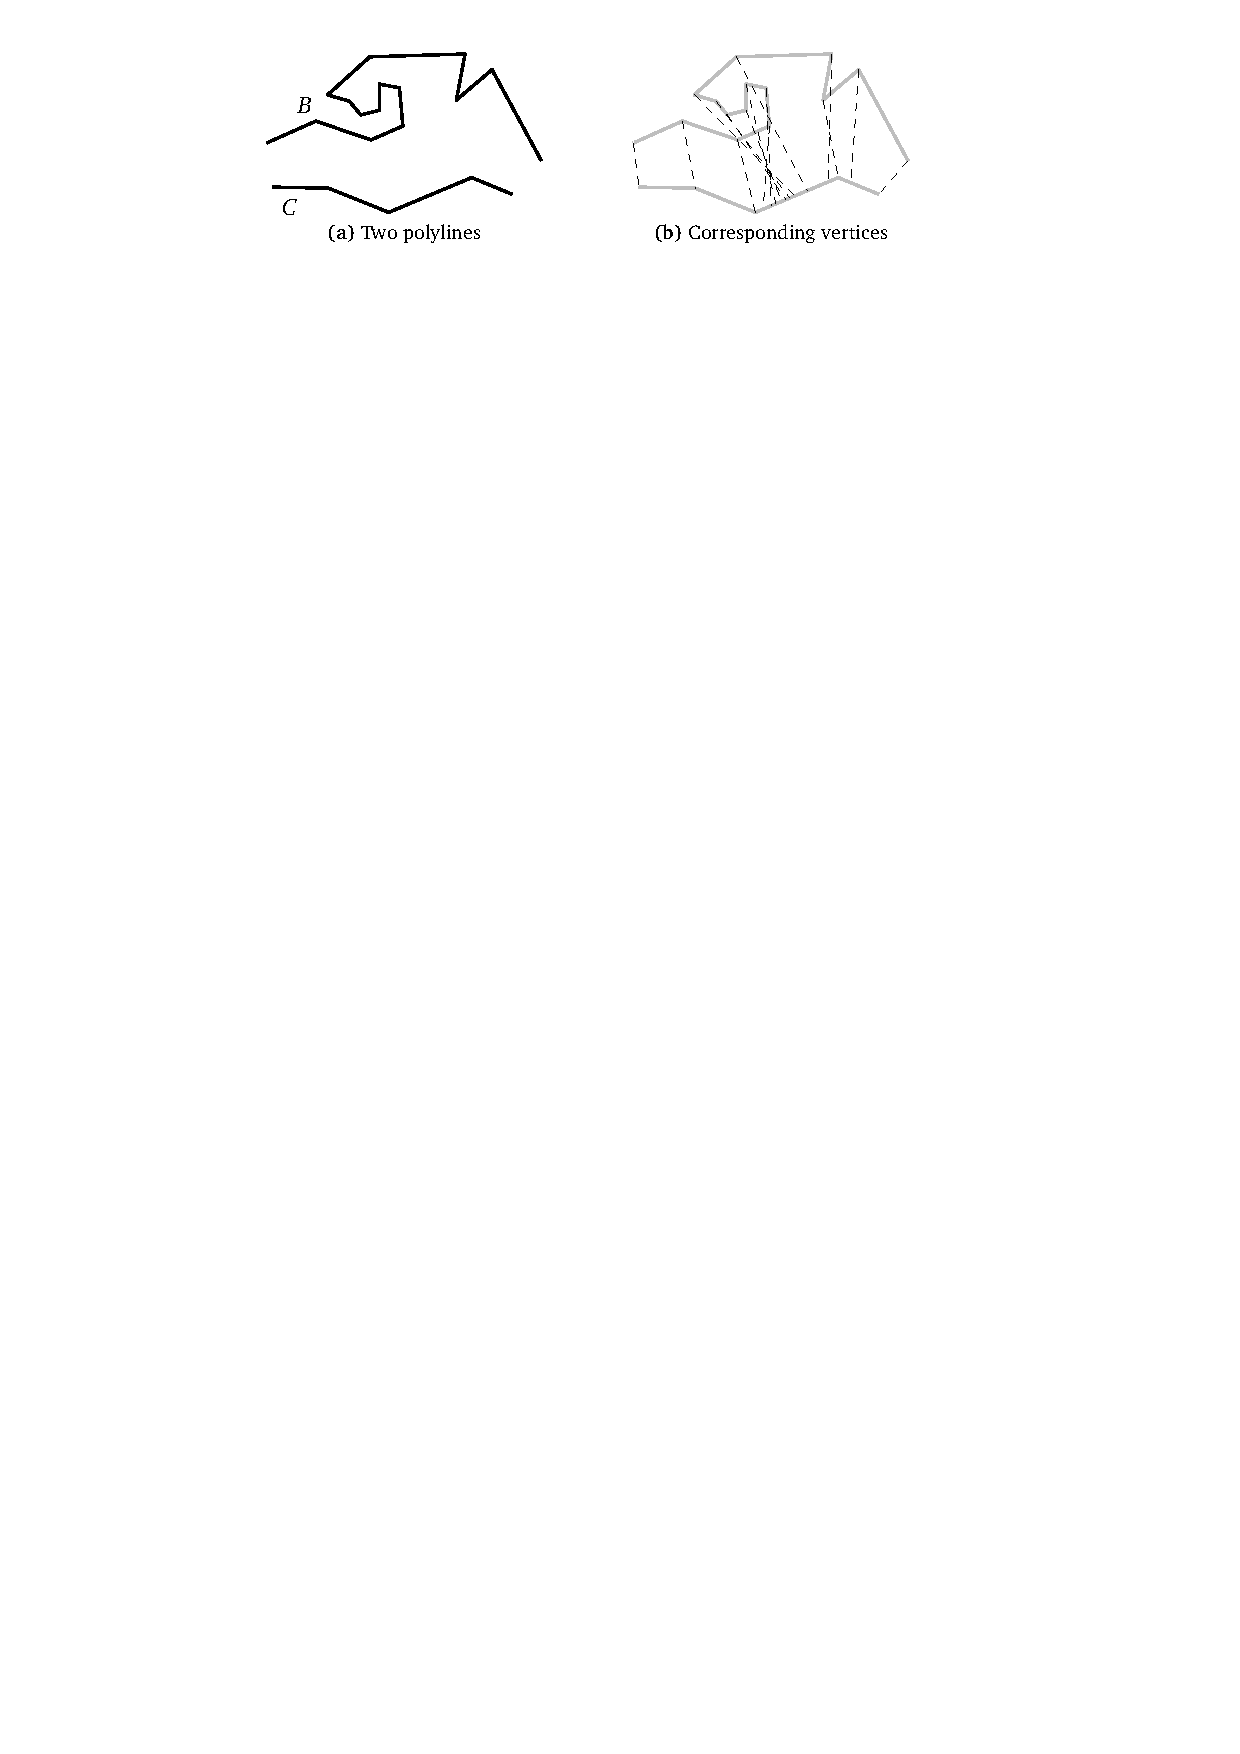
\includegraphics[page=1]{Morph_CaseStudy_Artificial}
	\caption{A dataset used in our experiments.}
	\label{fig:Morph_Data}
\end{figure}


\begin{figure}[tb]
	\centering	
	\includegraphics[page=2]{Morph_CaseStudy_Artificial}
	\caption{Morphing based on 
		straight-line trajectories (left) and
		based on our method (right).}
	\label{fig:Morph_Comparison}
\end{figure}

Unfortunately, there are still problems with our method. 
First, if we define the corresponding vertices 
between the polylines 
with a simple linear interpolation algorithm
(as shown in \fig\ref{fig:Morph_Undesirable}a), 
then we will obtain undesirable results 
when morphing polyline~$C$ to polyline~$B$ 
based on LSA 
(see \fig\ref{fig:Morph_Undesirable}b for example).

\begin{figure}[tb]
	\centering	
	\includegraphics[page=3]{Morph_CaseStudy_Artificial}
	\caption{An undesirable result based on our LSA.}
	\label{fig:Morph_Undesirable}
\end{figure}

Second, we may have self-intersections for some instances.
\fig\ref{fig:Morph_DataComplex} shows such an example,
where we have several self-intersections at time~$t=0.5$.  
We should try to develop some techniques 
to avoid this problem.

Third, sometimes the iterative process
(see \sect\ref{sec:Morph_Iterative})
does not stop because the norm of corrections~$\hat{x}(t)$
(see \eq\ref{eq:Morph_CoordinatesCorrections})
does not converge to value~$0$.
The reason is probably that
the polylines contain very short edges. 
\fig\ref{fig:Morph_ExtraVertices} shows such a strange result. 
For the corresponding vertices shown in 
\fig\ref{fig:Morph_DataComplex}b, 
we add an extra pair of corresponding vertices 
presented by the black curve in 
\fig\ref{fig:Morph_ExtraVertices}a.
The two extra vertices are very close to 
one of the pairs of corresponding vertices. 
Now, we have a pair of very short corresponding segments.
Because of that, our LSA generated a strange polyline 
at time~$t = 0.83$.
\fig\ref{fig:Morph_ExtraVertices}b shows the result, 
where the circle represents the extra vertex 
on the strage polyline.
By comparison, our LSA generated a correct polyline 
when we did not add the extra pair of vertices.
\fig\ref{fig:Morph_ExtraVertices}c shows the result, 
where the square represents the extra vertex 
on the correct polyline.
Moreover, our LSA does not converge 
at time~$t = 0.90$ when we have the extra vertices.

\begin{figure}[tb]
	\centering	
	\includegraphics[page=4]{Morph_CaseStudy_Artificial}
	\caption{Some self-intersections generated by our LSA.}
	\label{fig:Morph_DataComplex}
	%	
\par\vspace{\intextsep} %Leave a gap between the two figures
	%
	\centering	
	\includegraphics[page=5]{Morph_CaseStudy_Artificial}
	\caption{A strange result by our LSA.}
	\label{fig:Morph_ExtraVertices}
\end{figure}

\subsection{Case study on real data}
\label{sec:Morph_CaseStudy}

We tested our method on a part of the coastline of China 
(see \figs\ref{fig:Morph_RealData}a 
and~\ref{fig:Morph_RealData}d). 
The scale of the source polyline is~$1:5{,}000{,}000$,
the length is~$1{,}002\,$km, 
and the number of vertices is~$233$; 
the scale of the target polyline is~$1:30{,}000{,}000$, 
the length is~$605\,$km, 
and the number of vertices is~$66$. 
%
\figs\ref{fig:Morph_RealData}b and~\ref{fig:Morph_RealData}c
show the morphing results
at times~$t = 0.25$ and~$t = 0.75$,
where the prescribed vertices are marked by dots. 
Overall, we got nice results, 
but there are still some problems. 
In region~$R_{1}$, the two segments almost 
intersect at time~$t = 0.25$; 
in region~$R_{2}$, 
the ``bend'' first expands and then shrinks. 
The two phenomena are not appropriate. 
There are two reasons for both problems. 
First, the changes (decrease or increase) of the angles 
are faster than needed. 
Second, the decreases of the lengths are slower than needed. 
Both reasons tend to make a bend expand and then shrink. 
To solve this problem, we need a better model to 
simulate the changes of angles and edge lengths,
rather than use \eqs\ref{eq:Morph_AngleConstraints}
and~\ref{eq:Morph_LengthConstraints}.

\begin{figure}[tb]
	\captionsetup[subfigure]
	{justification=centering,font=normalsize}
	\begin{subfigure}[b]{\textwidth}
		\centering
		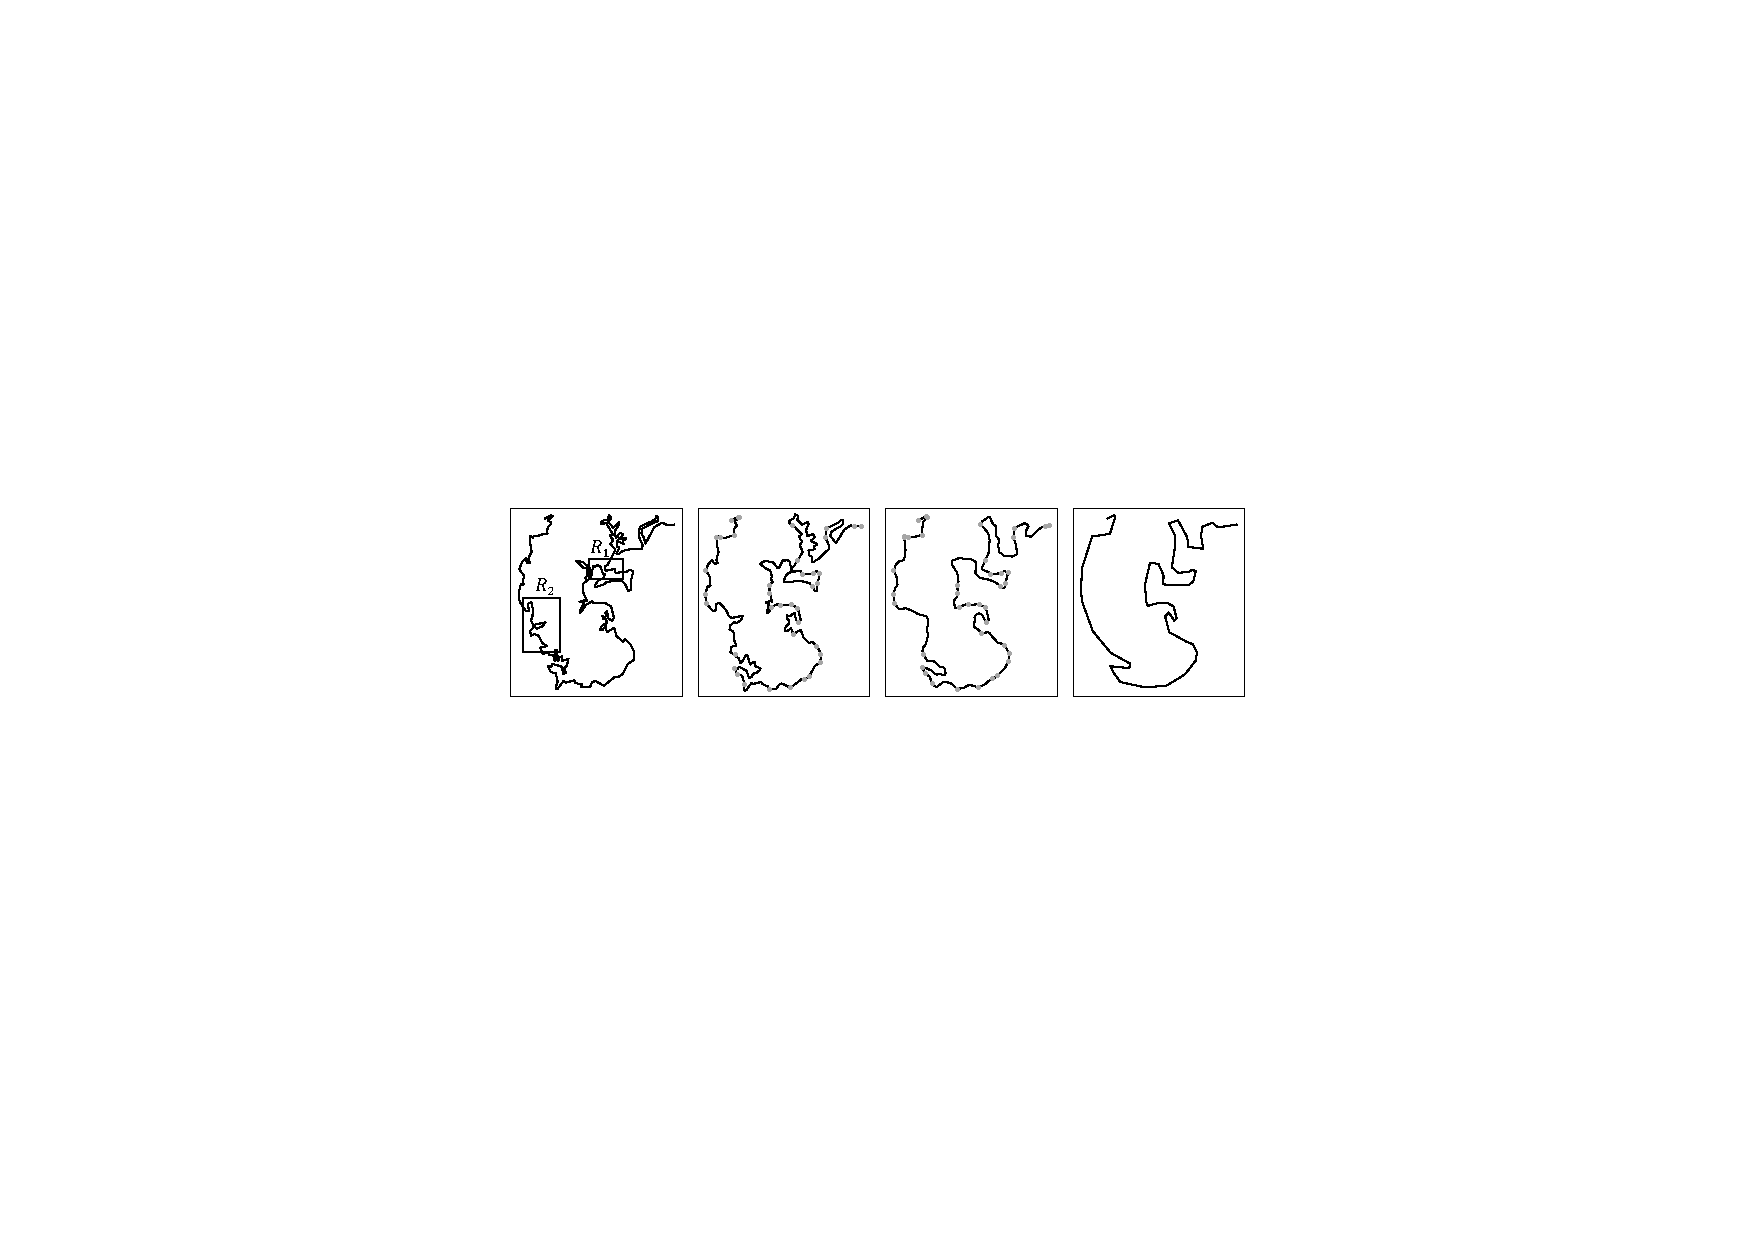
\includegraphics{Morph_CaseStudy_Real}
		\caption{
			\textbf{(a)} Source polyline~~~~~~~~
			\textbf{(b)} $t=0.25$~~~~~~~~~~~~~~
			\textbf{(c)} $t=0.75$~~~~~~~~~
			\textbf{(d)} Target polyline}
	\end{subfigure}
	\caption{Case study on real data.}
	\label{fig:Morph_RealData}
\end{figure}

\section{Concluding Remarks}
\label{sec:Morph_Conclusion}

We have introduced a method for morphing polylines 
that tries to linearly change 
the angles and the edge lengths over time. 
Our approach is based on LSA 
and can handle soft and hard constraints. 
Our first results are promising. 
Still, there are open problems. 
In particular, we have to ensure that 
our method always converges to a good solution. 
We also aim to model more constraints, 
for example, to avoid self-intersections. 
Besides, a further topic is 
to combine morphing and simplification.







